% DGEMV
Our first attempt at making a realistic application recoverable was an
iterative dense matrix-vector multiply (DGEMV) code. This application
repeatedly multiplies a vector by a constant matrix. Since the matrix is
constant, the only state that needs to be preserved is the vector and the last
successful iteration. This makes DGEMV somewhat of a best-case scenario for
traditional recovery schemes. The state is a single large allocation that
changes entirely on each iteration. In the following experiments, our RVM
implementation is compared with a manual serialization scheme that writes to
SSD's on our experimental system. The matrix was chosen to be of dimension
1Mx100 with 100 iterations in order to maximize the critical state and stress
the recovery schemes.

%XXX Graphs go here

In figure \ref{fig:dgemv_total_time_commit} we vary the commit rate (in terms
of iterations) from 1 (every time) to 100 (only one commit) without failures.
This essentially measures the overhead caused by recovery. In all cases, RVM
introduces less overhead. This is likely due to the efficient nature of RVM
checkpoints. More interesting, however, is when we introduce failures. In
figure \ref{fig:dgemv_total_time_fail}, we always commit on each iteration, but
inject failures after different numbers of iterations (from each iteration up
to a single failure). In this case, the file-based backend is faster than RVM
for high failure rates, but slower with low failure rates. We believe this is
due to a higher startup cost for the file-based approach. It also demonstrates
that reading a relatively large, sequential file from an SSD is very performant
and competes will with RDMA. We believe that further optimizations in the RMEM
layer could make up some of this difference, see Section~\ref{sec:conclusion}
for some possible performance enhancements.

\begin{figure}[t!]
\begin{center}
\resizebox{\columnwidth}{!}{%
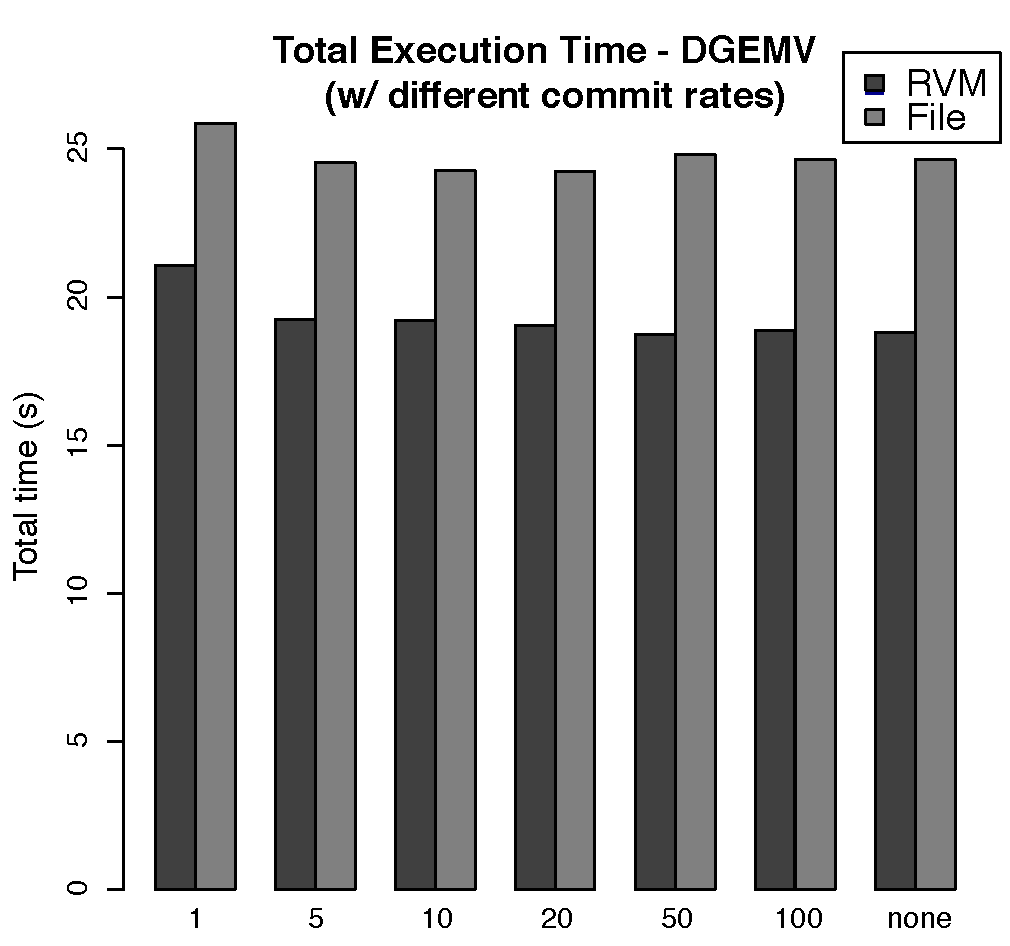
\includegraphics[scale=0.30]{graphs/dgemv_total_time_commit.pdf}
}
\end{center}
\caption{Total time of DGEMV application when committing at different rates}
\label{fig:dgemv_total_time_commit}
\end{figure}

\begin{figure}[t!]
\begin{center}
\resizebox{\columnwidth}{!}{%
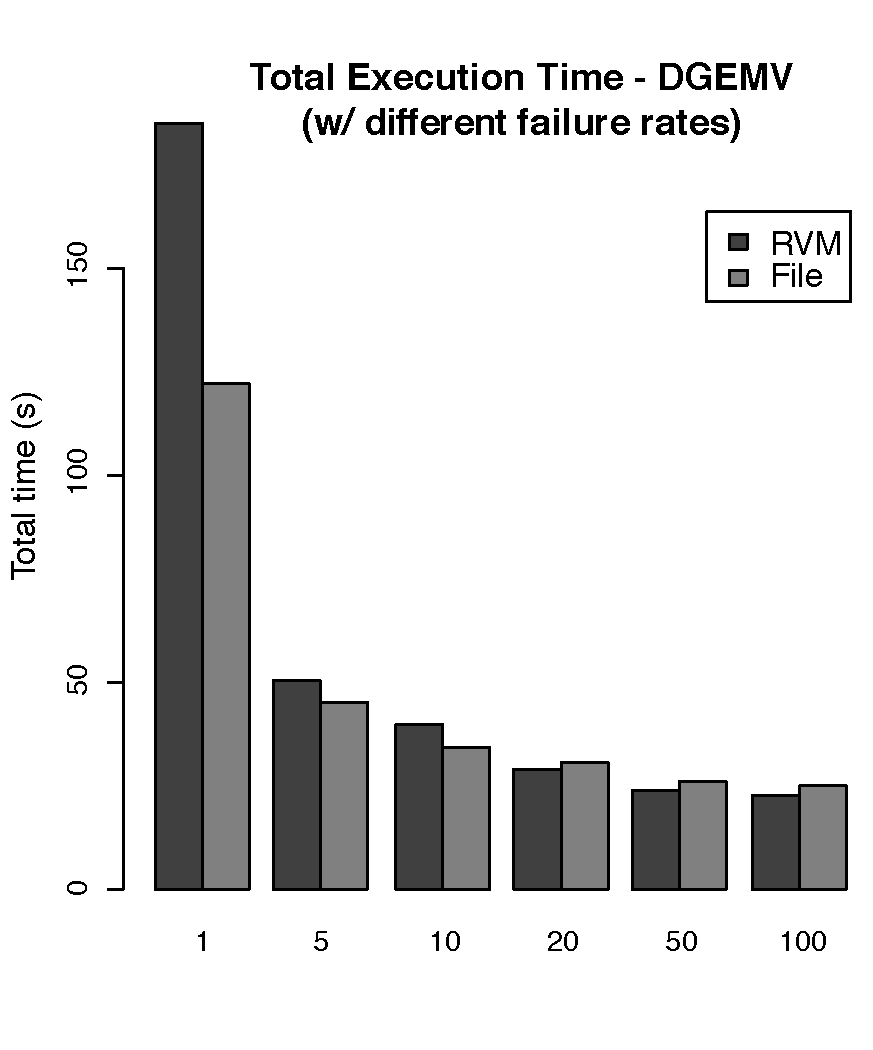
\includegraphics[scale=0.30]{graphs/dgemv_total_time_fail.pdf}
}
\end{center}
\caption{Total time of DGEMV application when failing/recovering at different rates}
\label{fig:dgemv_total_time_fail}
\end{figure}

